\section{システム概要}
システムの概要に関して述べる.
システムの全体概要は図 \ref{fig:system_summary}のようになっている.
本システムはクライアント部,バッチ処理部,データベース部の3部構成である.
各構成ごとに役割と機能の概要を説明する.
最後に処理の流れを述べる.

\begin{figure}[h]
  \centering
  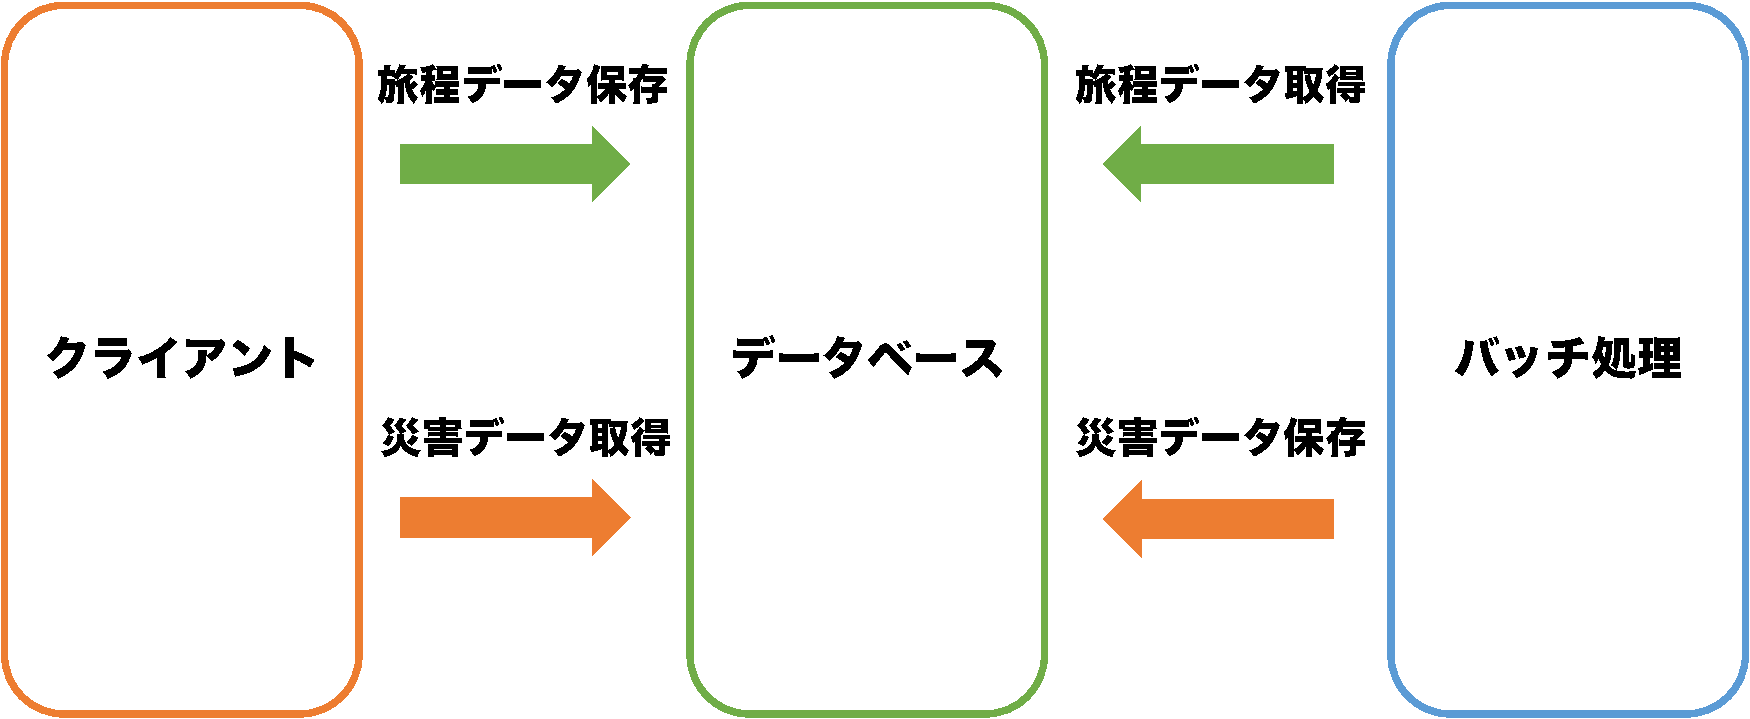
\includegraphics[height=6cm]{figure31.pdf}
  %\vspace{-3mm}
  \caption{システムの全体概要図}
  \label{fig:system_summary}
  %\vspace{2mm}
\end{figure}

\subsection{クライアント部}
クライアント部はこのシステムにおけるユーザインタフェースの役割を持つ.
旅程データの入力機能と注意情報を提供する機能がある.
具体的にはスマートフォンのアプリケーションを開発した.

\subsubsection{旅程データの入力機能}
ユーザはまず旅程のタイトルと期間を入力し,旅程パッケージを作成する.
旅程パッケージとは旅程データを1つにまとめたものである.
旅程データには,場所データと交通機関のデータの2種類が存在する.ユーザはこの2種類のデータで旅程を構築する.
ユーザは訪れる予定の場所や利用する予定の交通機関の位置情報を,予定時刻とともに入力インタフェースを通して入力する.
位置情報は両方の種類においても都道府県と市区町村名の名称である.
インタフェースは旅程パッケージごとに入力されたデータをデータベースへ保存する.
保存する際には旅程パッケージにクライアントidを付与する.

\subsubsection{注意情報提供機能}
第1章で定義したストック情報とフロー情報をユーザに提供する.
旅程データの入力機能にて事前に入力した旅程データのうち,災害の影響を受けると判断された旅程データを表示する.
その際に影響を受ける災害の種類と可能性の確率を提供する.
さらに,ユーザに対して災害の種類ごとにその現象と対処法についての情報を提供する.
また,影響を受ける旅程データが交通機関である場合,災害の可能性を交通機関が運休する可能性として情報を提供する.
その際に,運休によって起こる現象についての情報を提供する.

\subsection{データベース部}
データベース部はこのシステムにおけるデータを管理する役割を持つ.
データを保存する機能とデータを提供する機能がある.
具体的にはクラウドデータベースを利用した.

\subsubsection{データ保存機能}
ユーザがクライアント部で入力した旅程データを旅程パッケージごとに保管する.
また,バッチ処理部で旅程データと紐付けられた注意情報も保管する.

\subsubsection{データ提供機能}
クライアント部の要求には,旅程パッケージに付与されているクライアントidを条件にデータを提供する.
バッチ処理部の要求には,旅程データの予定時刻を条件にデータを提供する.

\subsection{バッチ処理部}
バッチ処理部は,旅程データが災害の影響を受けるか監視する役割を持つ.
気象庁が定期的に公表する,注意情報を取得して,ユーザがクライアント部で入力した旅程データと照合する.
災害の影響を受ける旅程データがあれば注意情報と旅程データを紐づけてデータベースに保存する.
旅程データを作成したクラアントに通知する指示を出す.
具体的にはPythonのプログラムを作成した.

\subsubsection{気象庁から注意情報の取得}
注意情報とは災害の影響を受ける可能性と予定時刻,発表地域で構成される情報である.
この情報は気象庁から定期的にweb上で発表されている.
その時刻に合わせてバッチ処理が実行され,注意情報を取得する.

\subsubsection{旅程データの取得}
注意情報の予定時刻と重なる旅程データを検索する.
データベース部から旅程データを取得する.

\subsubsection{注意情報と旅程データを照合}
注意情報の予報時刻に当てはまる旅程データを抽出した後,旅程データの場所情報をもとに,注意情報を関連付けて保存するか判断する.
注意情報の発表地区は気象庁が独自に定めている,各都道府県の市区町村のまとまりである.
注意情報に災害の予測が記載されている場合,旅程データの位置情報から発表地区に属するデータを抽出し,注意情報を旅程データと紐付ける.
災害の影響を受けると判断された旅程データはデータベースに保存する.
もし注意情報に災害の予測が記載されてなければ何もしない.


\subsubsection{クライアント部へ通知指示}
災害の影響を受けると判断された旅程データを作成したクライアントに通知を送信するよう指示を出す.
しかし,評価実験をするにあたって評価指標とは関連がない機能であったことと,コスト削減のため本研究ではクライアント部からの通知機能を実装した.

\subsection{処理の流れ}
システムの処理の流れについて述べる.
図 \ref{fig:activity}にアクティビティを示す.

\begin{quote}
  \begin{enumerate}
    \item 旅程データの入力(クライアント部)
    \item 旅程データの保存(データベース部)
    \item 気象庁から注意情報の取得(バッチ処理部)
    \item 旅程データの取得(バッチ処理部)
    \item 旅程データの提供(データベース部)
    \item 注意情報と旅程データを照合(バッチ処理部)
    \item 注意情報の保存(データベース部)
    \item クライアント部へ通知指示(バッチ処理部)
    \item 通知(クライアント部)
    \item 注意情報の提供(データベース部)
    \item 注意情報提供(クライアント部)
  \end{enumerate}
\end{quote}

\begin{figure}[H]
  \centering
  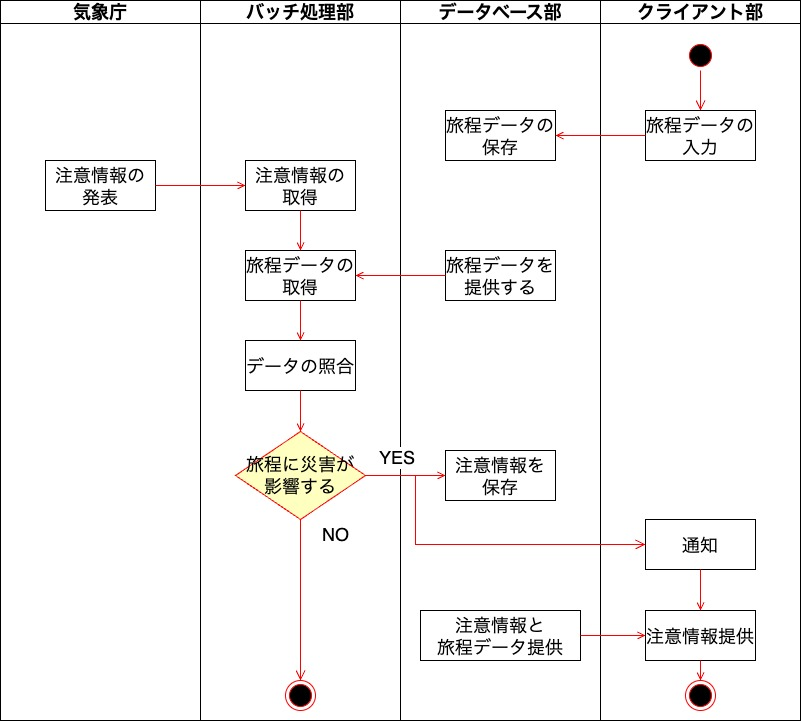
\includegraphics[height=10cm]{figure32.jpg}
  %\vspace{-3mm}
  \caption{システムのアクティビティ図}
  \label{fig:activity}
  %\vspace{2mm}
\end{figure}